% !TeX root = ../main.tex
\chapter{系統實驗與結果討論}

    本章將說明本論文研究所提出之系統的實作與實驗。
首先說明系統各角色之實作細節,並於接續章節說明實驗與結果討論。

\section{系統實作}

    本章節將說明本論文研究所提出的協定與硬體之實作,包含「會談終端」、「解封伺服器」
與供會談主持者用於與解封伺服器通訊的「行動應用程式」。

\subsection{會談終端}

    會談終端包含多個組件,其概念驗證實作硬體組成如圖\ref{fig:mbox}。

\begin{figure}[H]
    \centering
    \includegraphics[width=1.0\textwidth]{mbox}
    \caption{會談終端概念驗證實作}\label{fig:mbox}
\end{figure}


\paragraph{超音波麥克風干擾器}

    如圖\ref{fig:mbox}\nameref{fig:mbox}中左下紫色實線多邊形方框所示。
此超音波麥克風干擾器為參考Yuxin Chen,  Huiying Li 等人的實作\cite{chen2020wearable}。
包含一 Arduino Micro 用於產生於$24k\sim26k$之間的偽隨機數與控制周邊裝置。
包含一波形產生器 AD9833,透過SPI與Arduino Micro溝通取得偽隨機數,產生介於$24khz\sim26khz$之間正弦波。
包含一數位放大器 HW-104,用於放大訊號產生器產生的訊號以驅動超音波發射器。
包含一超音波發射器,產生介於$24khz\sim26khz$之間的超音波。
此超音波麥克風干擾器於系統時脈$16Mhz$的單晶片控制器中,每 $2ms$ 產生新的偽隨機數,使其生成干擾超音波。

\paragraph{錄音麥克風}

    如圖\ref{fig:mbox}\nameref{fig:mbox}中左上紅色虛線圓框所示。
包含一USB數位駐極電容式麥克風 Saramonic LavMicro U3A。
用於錄製受超音波麥克風干擾器干擾的會談對話聲音記錄 (\DEFrecJ),
與產生純超音波麥克風干擾器於麥克風的響應輸出(純噪音)之聲音記錄 (\DEFrecN)。

\paragraph{物理控制介面}

    提供會談參與者操作與會談終端互動,獲得外部觸發事件。

\paragraph{人機互動介面}

    用於傳遞會談的元資料與系統狀態提示給會談參與者。

\paragraph{運算控制核心與網路介面}

    周邊裝置控制與邏輯運算核心,用於處理聲音記錄、執行加密與解封伺服器通訊等運算工作。



\subsection{解封伺服器}


\subsection{行動應用程式}


\section{系統實驗}

\subsection{超音波麥克風干擾器之干擾效果分析}

    會談聲音與麥克風干擾器產生的干擾之信噪比下,干擾效果的分析。
包含人耳聽感,與語音識別。


\subsection{主動式噪音消除效果分析}

    會談聲音與麥克風干擾器產生的干擾之信噪比下,噪音消除效果分析。
包含人耳聽感,與語音識別。


\subsection{聲音樣本離散時間推估演算法}

    此演算法的執行前後聲波比對圖,與執行過程數值的變化。


\subsection{解封會談聲音記錄分析性能分析}

    伺服器獲得授權後,執行聲音樣本離散時間推估演算法與主動式噪音消除來還原產生有效的會談聲音紀錄,
其錄音長度與執行時間的時間複雜度性能分析。


\section{實驗結果與討論}

    本研究所設計之系統可以確保 Server 在 Running {\it Meeting Session}結束後,
直到成功解封 ({\it Unseal})之前,\DEFrecREV 保有機密性。

\begin{figure}[H]
    \centering
    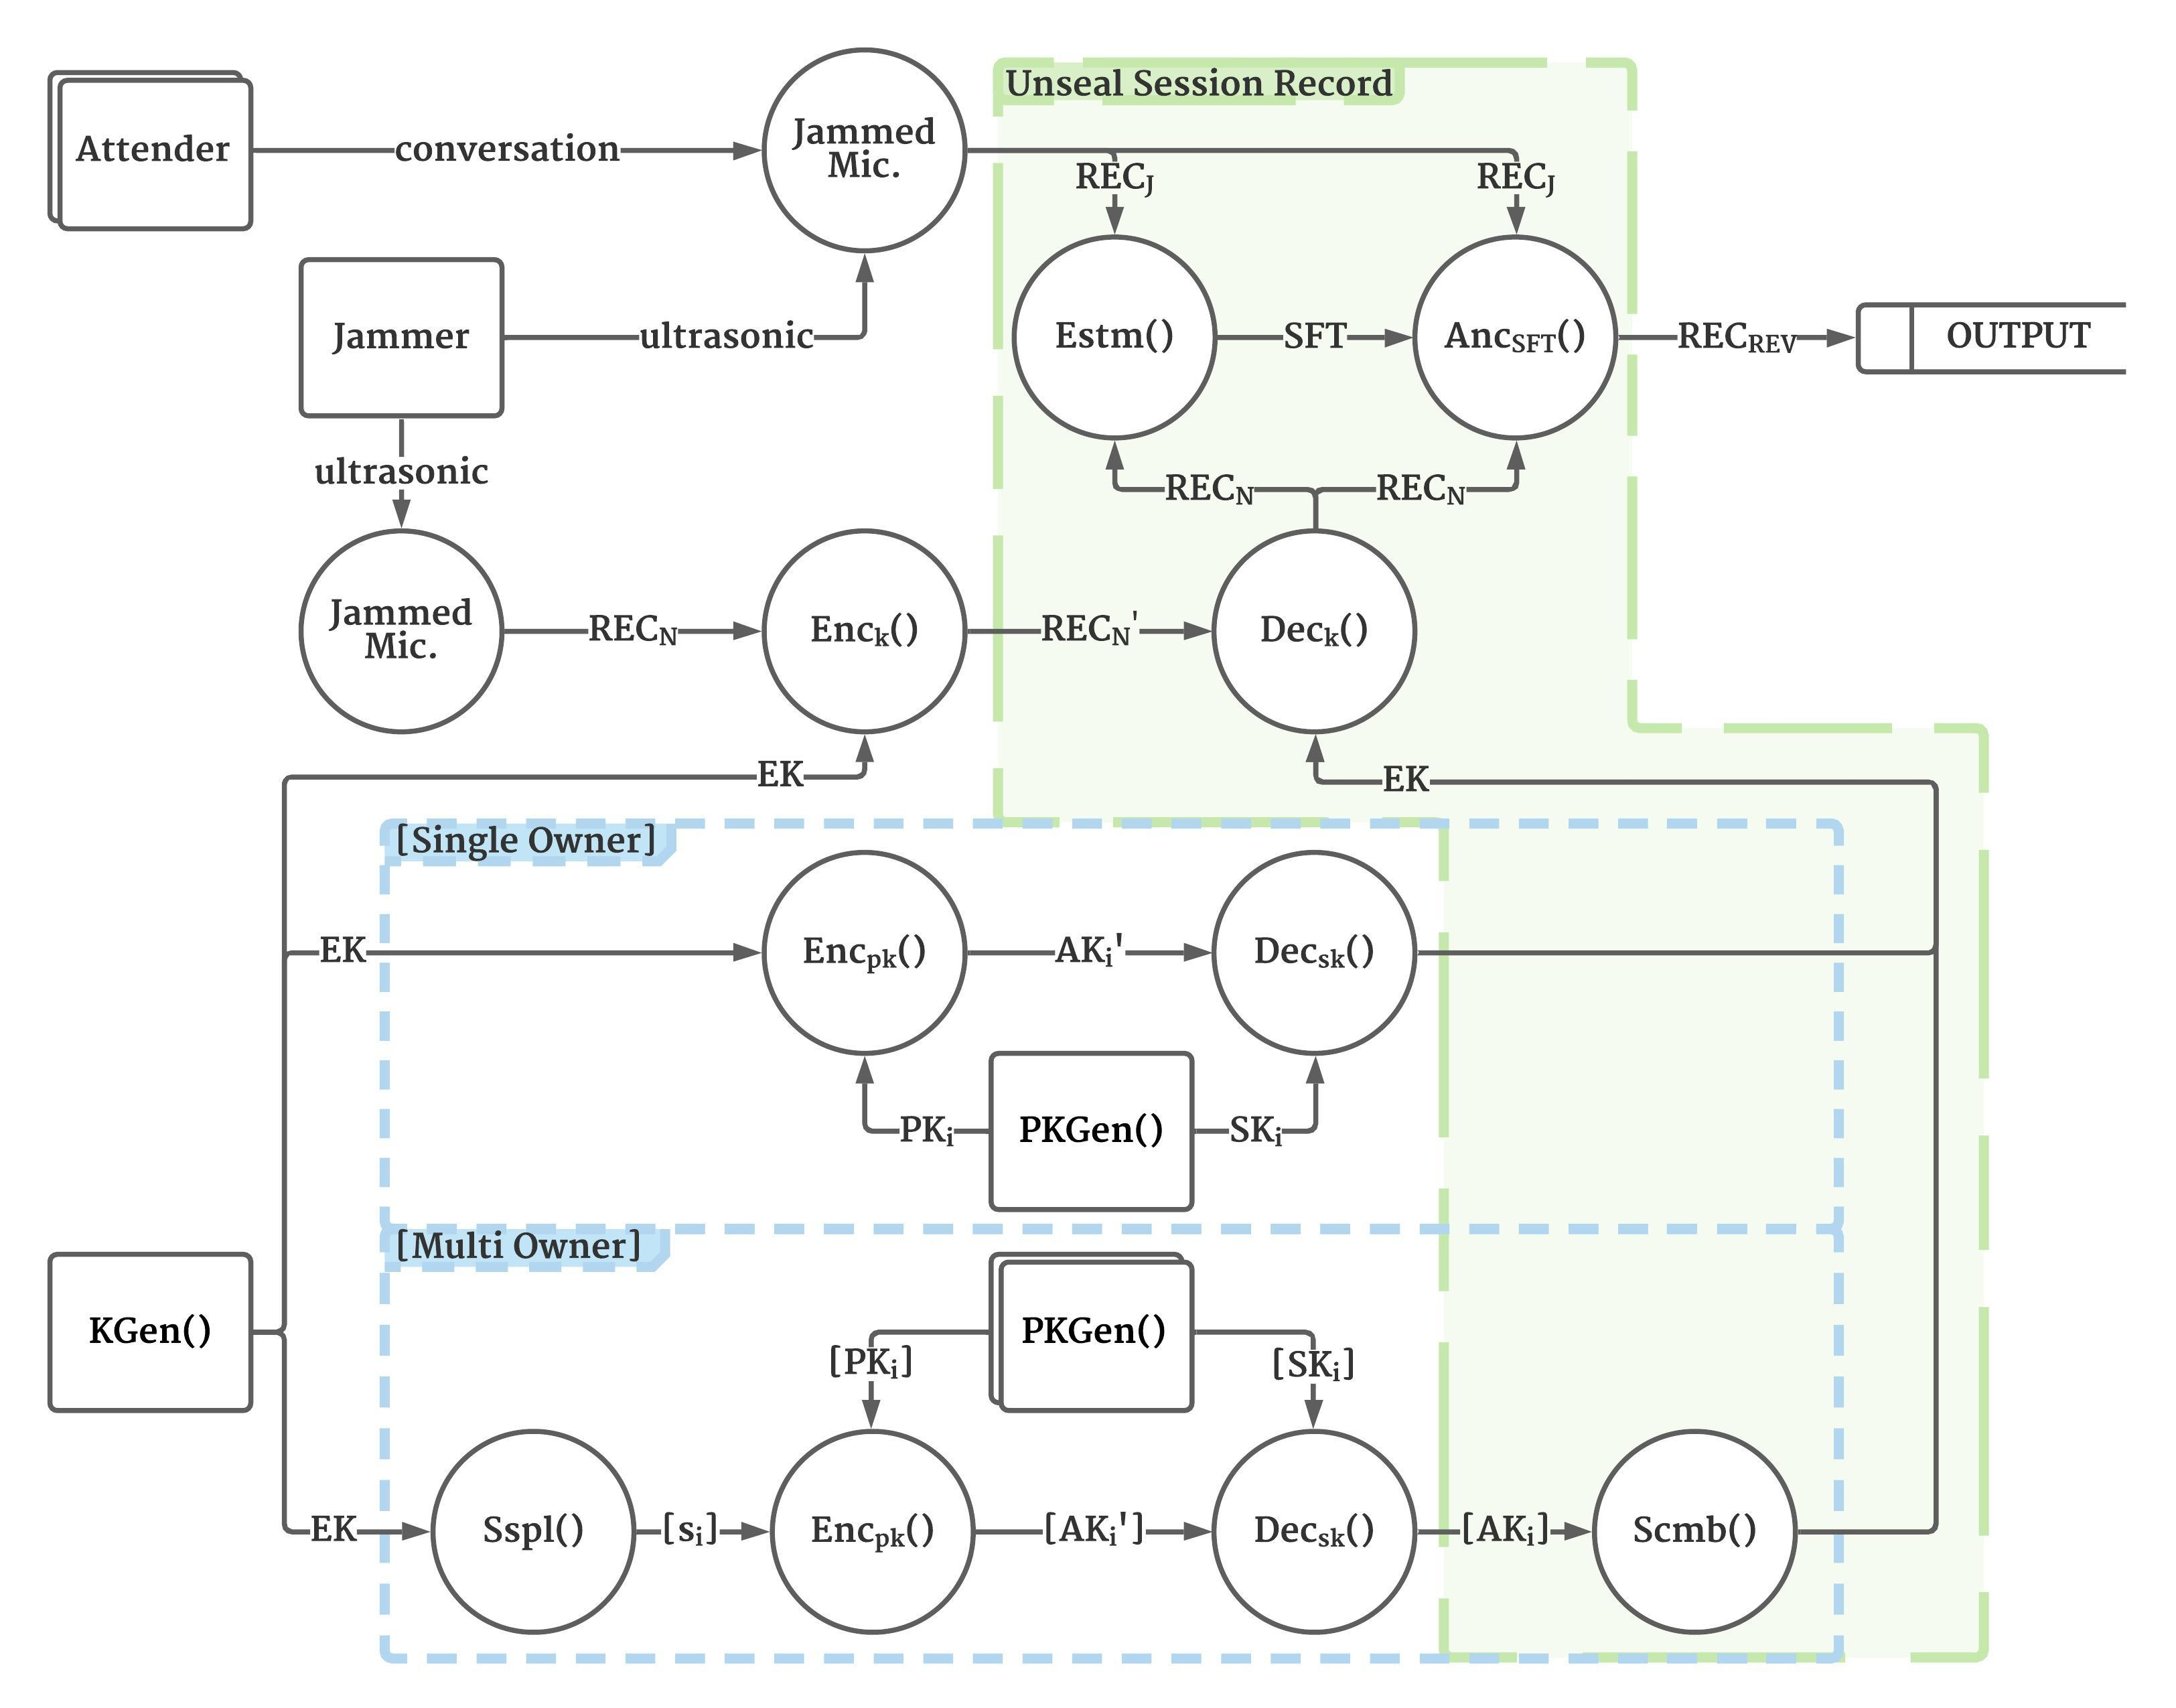
\includegraphics[width=1.0\textwidth]{system-data-flow}
    \caption{系統資料流程圖}\label{fig:system-data-flow}
\end{figure}